% This is samplepaper.tex, a sample chapter demonstrating the
% LLNCS macro package for Springer Computer Science proceedings;
% Version 2.20 of 2017/10/04
%
% This is samplepaper.tex, a sample chapter demonstrating the
% LLNCS macro package for Springer Computer Science proceedings;
% Version 2.20 of 2017/10/04
%
\documentclass[runningheads]{llncs}
%
\usepackage{ctex}
\usepackage{subfigure}
\usepackage{amsmath}
\usepackage{booktabs} % For pretty tables
\usepackage{caption} % For caption spacing
\usepackage{subcaption}
% For sub-figures
\usepackage{longtable}
\usepackage{graphicx}
\usepackage{pgfplots}
\usepackage[all]{nowidow}
\usepackage[utf8]{inputenc}
\usepackage{tikz}
\usetikzlibrary{er,positioning,bayesnet}
\usepackage{multicol}
\usepackage{algpseudocode,algorithm,algorithmicx}
\usepackage{minted}
\usepackage{hyperref}
\usepackage{geometry}
\usepackage[inline]{enumitem} % Horizontal lists
% Used for displaying a sample figure. If possible, figure files should
% be included in EPS format.
%
% If you use the hyperref package, please uncomment the following line
% to display URLs in blue roman font according to Springer's eBook style:
% \renewcommand\UrlFont{\color{blue}\rmfamily}

\newcommand{\card}[1]{\left\vert{#1}\right\vert}
\newcommand*\Let[2]{\State #1 $\gets$ #2}
\definecolor{blue}{HTML}{1F77B4}
\definecolor{orange}{HTML}{FF7F0E}
\definecolor{green}{HTML}{2CA02C}

\pgfplotsset{compat=1.14}

\renewcommand{\topfraction}{0.85}
\renewcommand{\bottomfraction}{0.85}
\renewcommand{\textfraction}{0.15}
\renewcommand{\floatpagefraction}{0.8}
\renewcommand{\textfraction}{0.1}
\setlength{\floatsep}{3pt plus 1pt minus 1pt}
\setlength{\textfloatsep}{3pt plus 1pt minus 1pt}
\setlength{\intextsep}{3pt plus 1pt minus 1pt}
\setlength{\abovecaptionskip}{2pt plus 1pt minus 1pt}
\geometry{left=2cm,right=2cm}

\begin{document}
%
\title{多方法高光谱图像分割效果比较}
%
%\titlerunning{Abbreviated paper title}
% If the paper title is too long for the running head, you can set
% an abbreviated paper title here
%
\author{3220210653 
王澳}
%
%\authorrunning{F. Author et al.}
% First names are abbreviated in the running head.
% If there are more than two authors, 'et al.' is used.
%
\institute{Beijing institute of technology
\url{https://github.com/Crescent-Ao}}
%
\maketitle              % typeset the header of the contribution
%
\begin{abstract}
高光谱图像不同于传统的可见光图像,它具有大量的光谱信息和光谱维度,因此较多光谱维度存在大量的信息冗余,各个光谱维度的相关性较高,因此特征空间降维和相应的光谱特征提取是高光谱图像理解解译的必要手段。从降维手段上来看,主要分为有监督和无监督两种主要方式,其中有监督方式以LDA,LLE,还有以集成学习为主的算法提取的Gini系数(xgboost和随机森林),无监督方式主要是以PCA方式为主。从特征提取手段上来看,传统的机器学习必须通过较好的特征工程,来提取数据的特征,包括特征融合,拆分,映射等方面,回到图像中来,LBP,GLCM,gabor,SIFT等手段,都是特征工程的主要部分。另一方面,随着深度学习的发展,特征提取和相应的分类器的实现都可以通过数据的反向传播来获取最适宜的参数。此次作业中设计了两种方式来进行高光谱图像分割效果比较,一是通过人工特征提取的xgboost高光谱图像分割,二是基于注意力机制的卷积神经网络的高光谱图像分割。实验结果表明,深度学习和级联多特征高光谱图像分类在精度和鲁棒性橡胶而言,两者的精度和鲁棒程度大致相当。但是深度学习Patch块信息的提取,是利用了大量的先验信息的存在。而对于传统的特征提取中,通过手动提取相关特征,则更意味着特征的获取的不稳定性和主观性。因此两种方法各有利弊,都有其各自存在的问题

\keywords{ SVM  \and XGBOOST classification   \and LDA \and Deep learning}
\end{abstract}
%
%
%
\section{数据阐述}
高光谱图像作为遥感领域的一项重大突破,在保留较高空间分辨率同时,其光谱分辨率有极大的提高,达到了纳米的数量级,可以用来探测和识别传统全色和多光谱遥感中不可探测的地物类别.与传统的多光谱遥感图像相比,高光谱遥感图像有着信息量大,光谱分辨率高等特点,这使得在描述与区分地物类别方面的能力有了大幅提高,进而为地物光谱信息的精确处理与分析提供了可能\cite{何同弟0高光谱图像的分类技术研究}。

本次实验选取的数据集来源于帕维亚大学上空的高光谱遥感图像处理,空间分辨率为$610 \times 340$,光谱维度为103,Flatten处理后,二维数据集的Shape为$20400 \times 103 $,有效标记点数为42776个,下图是光谱带之间的协方差矩阵的Heatmap,可以看出大量的光谱信息存在着冗余,因此降维和特征提取是必要的。
\begin{figure}
    \centering
    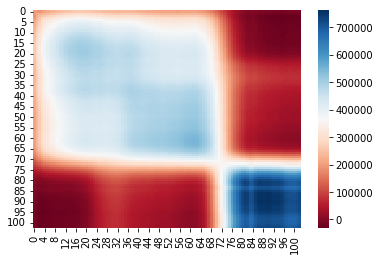
\includegraphics{cov.png}
    \caption{光谱协方差矩阵}
    \label{guan}
\end{figure}
\subsubsection{定量分析光谱的冗余程度}
为了进一步验证光谱数据的冗余程度,提出了一种基于随机森林和相关分析的定量分析方法。首先将K个类别的基尼系数计算出来,假设有K个类别的对应K个类别概率为$p_k$,如果是给定的样本D,假设有K个类别,第K个类别的数量为$C_k$,计算样本D的基尼系数为
\begin{equation}
    Gini(p) = \sum_{i=1}^Kp_k(1-p_k),Gini(D)=1-\sum_{i=1}^K\frac{\abs{C_K}^2}{\abs{D}^2}
\end{equation}
每个节点的基尼系数减去子几点的基尼系数计算的数据值被看做基尼减少。最后,所有相同
特征节点的上述值被衡量为基尼重要度,它的值将会在 0 到 1 之间,如果该值越大则代表该
特征越重要。当然,特征重要度也有之对一个的缺点,此类方法的缺点是算法倾向于选择有
大量数据的数字特征和分类特征。同时,在相关特征的选择上,它倾向于选择单一特征而忽
略第二个有较大相关重要度的特征,这往往会导致错误的结论。

随机森林的 Gini 指数同相关分析中相关系数融合。在归一化之后,分别给其赋予对应的权重。
由于随机森林的特征重要度,在分类问题中实现特征降维的效果更好,所以我们赋予其更多
的权重。而对应的相关分析得分,则赋予较小的权重。上述分析中,我们各自分析特征重要
度和相关分析的优缺点,随机森林的缺点是如果两个特征的相关程度较大就会倾向于选择一
个,而相关分析的存在正好克服这一缺点,从理论上来说特征得分也有其存在的意义。
\begin{equation}
    Feature\quad Score = Feature\quad importance \times \alpha_1 + Correlation\quad importance \times \alpha_2
\end{equation}
\begin{figure}[t]
\centering  %图片全局居中
\subfigure[特征得分的归纳统计值]{
\label{Fig.sub.1}
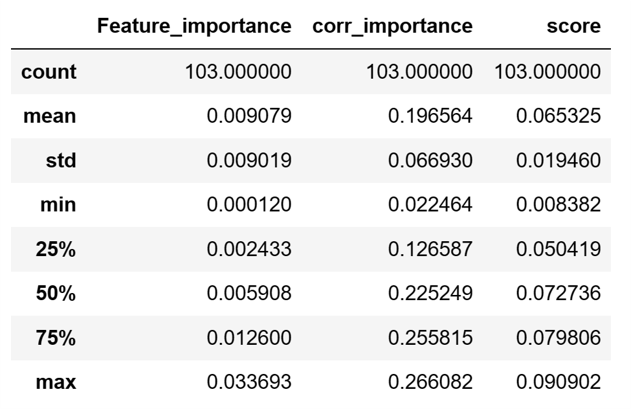
\includegraphics[width=8cm,height = 6cm]{feature_score_analysis.png}}\subfigure[特征得分的计算value]{
\label{Fig.sub.2}
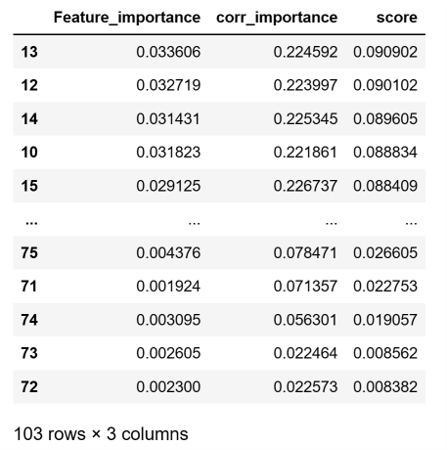
\includegraphics[width=8cm,height = 6cm]{feature_score.png}}
\caption{特征得分的归纳统计值}
\label{1}
\end{figure}
\begin{figure}
    \centering
    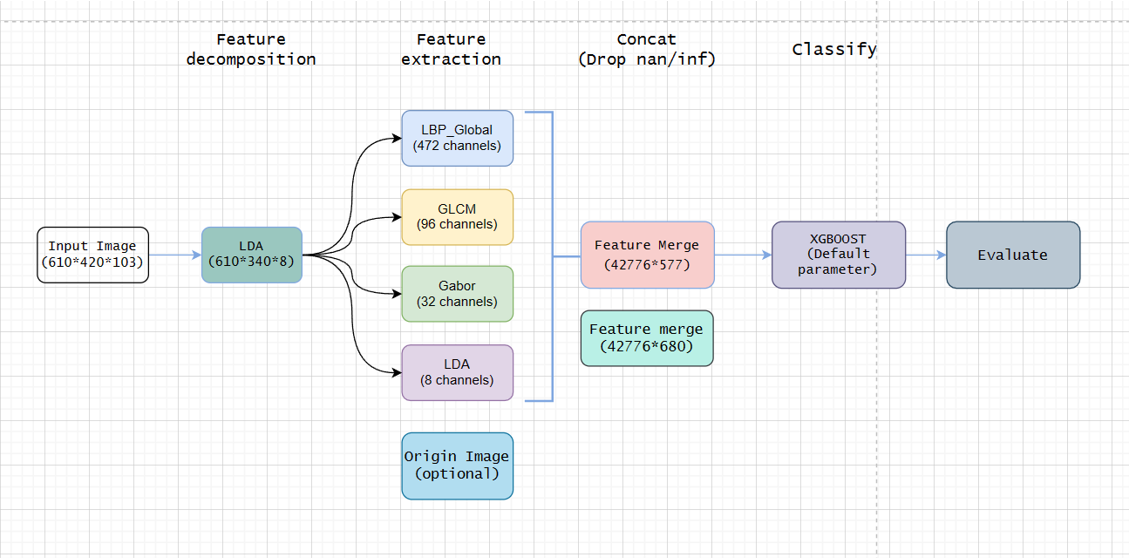
\includegraphics[width=18cm]{architecture.png}
    \caption{多特征级联高光谱图像架构}
    \label{fig:my_label}
\end{figure}
\section{多级联特征高光谱图像分类}
    上图展示了此次大作业的整体框架,主要是五个部分分别是特征降维,特征提取,特征级联及一些特征值的处理(包括丢弃特征中重复值,无穷值,缺失值,特征归一化等几个简单的处理方法),最后丢入分类器,本次选取的分类器是XGboost,最后进行评估的操作。
    
\subsection{降维}
由于高光谱图像包含数百个窄的连续带,因此频带(特别是相邻频带)之间通常具有强相关性。 为了增加所显示的信息量,通常将图像的维度降低到具有较高信息密度的较小的一组特征(例如,通过PCA和LDA两种方式)。
\subsubsection{弱分类器评估降维效果}
本次作业中选取了这两种方法,通过训练一个弱分类器即不做任何处理,分类器选择的主要模型是最基础的SVM模型,训练集和测试集的分割比例是50\%,评价指标分别是OA和AA、kappa系数三个指标。我们可以看出在相较于输入原始的图像,LDA方法较高的保存了图像的信息,最终的维度为8维。


弱分类的意义在于利用简单的分类器,来判断当前的降维效果,即检查当前的降维是否能够大量保留原始输入的特征图的信息密度,或者说弱分类的存在是为了避免下面特征提取的过程不是因为原始信息密度缺失而造成分类效果的指标较差。如果直接将降维后的数据送入分类器中,可见输入的特征越多输出的相应的结果就越好,PCA是三个维度而对应的8个维度的LDA明显是更好的,现在就只有两种方法,要不将原始的降维后的数据送入分类器,然后根据特征提取算法,获得更多通道数的特征。第二个,直接送入对应的分类器,由于XGBoost集成学习算法的特性,会自动根据当前的特征冗余来进行特征选取,因此对应的降维的过程实际上可以减少一步,直接输入对应的分类器来获取相应的结果。\\

\subsubsection{降维的处理方法}
基于高光谱图像的特征工程主要包括两个方面,分别是PCA和LDA处理,PCA是一种常见的非监督的降维方式,本次选取了三个特征.方差累计贡献率到达99.158\%。有监督的方式采用的是LDA方法,由于LDA方法生成的维度,总是标签总数减一的数量,因此对应的维度就是8维度,特别注意的是这里的降维是对42776个标记数据而言。但是LBP、GLCM和Gabor等等特征提取手段都是针对整幅图而言,所以将上述降维的模型参数保存下来。再通过对原始数据映射到对应的高维空间中,然后进行下面的特征提取的过程。
\begin{table}[]
\caption{降维方法比较}
\centering
\setlength\tabcolsep{25pt}
\label{tab:my-table}
\begin{tabular}{llll}
\toprule
Tr(50\%) & oa       & aa       & kappa    \\

\midrule
Origin  & 95.79670 & 93.94443 & 94.41312 \\
LDA     & 92.20984 & 90.19212 & 89.90751 \\
PCA     & 55.44230 & 32.84935 & 34.52481\\
\bottomrule
\end{tabular}
\end{table}

\begin{enumerate}
    \item 第一主成分 0.58300739 累计贡献率 0.58300739
    \item 第二主成分  0.35858552 累计贡献率 0.9415929
    \item 第三主成分0.04999 累计贡献率 0.99158291
\end{enumerate}
\begin{figure}[t]  %图片全局居中
\centering
\subfigure[PCA 图像]{
\label{Fig.sub.1}
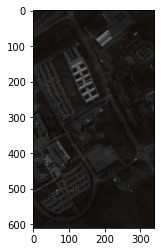
\includegraphics[width=4cm]{pca_figure.png}}\subfigure[LDA 图像]{
\label{Fig.sub.2}
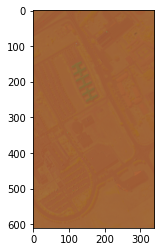
\includegraphics[width=
4cm]{lda_figure.png}}
\caption{降维的两种图像的展示}
\label{1}
\end{figure}
\subsection{特征提取}
特征提取方面使用了四个方向,4个尺度的gabor核,也就是Gabor核来进行相应的特征提取。也就是说降维之后的光谱维度,每一个gabor核会提取相应通道的特征,PCA输出三维,特征提取之后会新生成60维度的特征。LDA降维之后的输出是8维度,会生成160维度的特征,每一个维度送入到基础的分类器算法中(XGBOOST或者SVM算法中),然后进行分类。
注重介绍一下特征提取的三个部分,分别是LBP GLCM Gabor等三个特征提取的方法,同时在网络的训练中,我们发现将LDA放入原始的八个特征后,精度也会有所特征。同时,在回到之前的数据的数据降维的过程中,我们发现,将原始的图像送入分类器精度较降维后而未做特征提取有较大的提高。如果特征提取后,再将原始的图像堆叠进去,精度是否也会有较大的提升,具体的结果将在后面具体展示。
\subsubsection{单特征与级联多特征}
这个也是弱分类器的结果,我们发现通过级联特征的存在可以弥补单个特征的信息缺失,级联特征的存在使得信息互补提高了分类的准确度。给出部分的结论。较为有效的两个特征分别为GLCM和LDA原始特征,Gabor和LBP效果不是很明显。
\begin{figure}[t]
\centering  %图片全局居中
\subfigure[单特征分类]{
\label{Fig.sub.1}
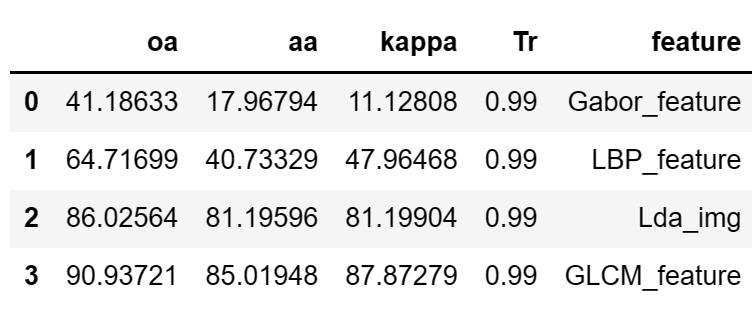
\includegraphics[width=8cm]{feature.png}}\subfigure[多特征分类]{
\label{Fig.sub.2}
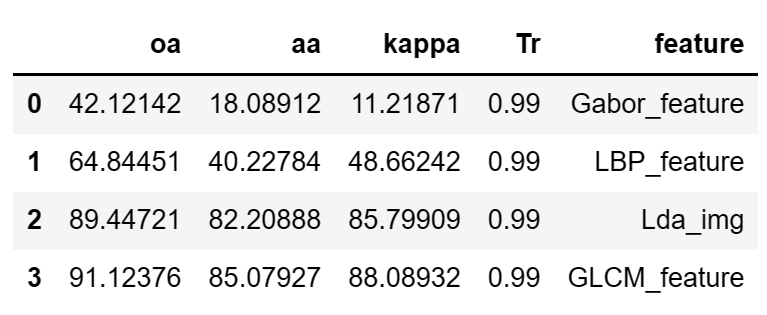
\includegraphics[width=8cm]{feature_concat.png}}
\caption{特征提取}
\label{1}
\end{figure}

\subsection{分类器介绍}
XGBoost是一个优化的分布式梯度提升库,旨在高效、灵活和便携。它在Gradient Boosting框架下实现机器学习算法。XGBoost 提供并行树提升(也称为 GBDT、GBM),可以快速准确地解决许多数据科学问题。相同的代码运行在主要的分布式环境(Hadoop、SGE、MPI)上,可以解决数十亿个示例之外的问题。
\begin{figure}
    \centering
    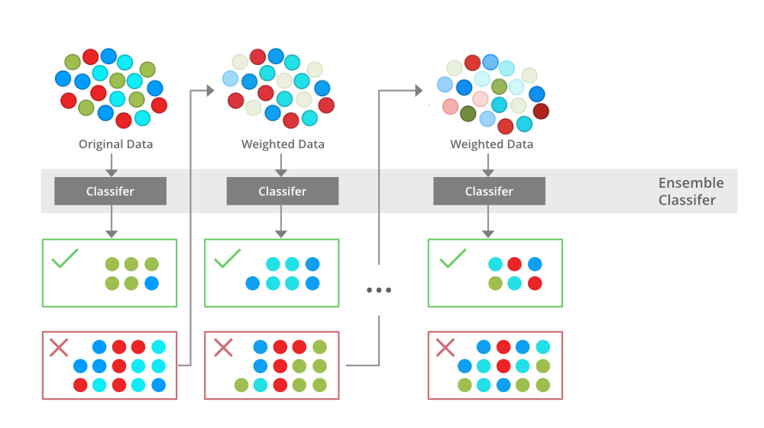
\includegraphics{1.png}
    \caption{XGBOOST}
    \label{fig:my_label}
\end{figure}
\subsection{模型评估}
\subsubsection{评价指标}
\qquad \textbf{kappa系数}用于一致性检验的指标,也可以用来衡量分类的效果。对于分类问题,一致性就是模型预测结果和实际分类结果是否一致。


\textbf{overall Accuracy}正确分类测试样本数/总的测试样本数


\textbf{AA}每个类的正确平均


\textbf{Each ACC} 每个类的准确度


具体的实现细节如下,通过设置sklearn的stratify参数,在数据集划分的过程中可以根据特征点在数据集的整体分布比例来进行数据的采样的过程,划分比例是6种比例来进行对应的数据划分的方法。数据输入前要进行对应的特征的标准化的处理,来加快对应的拟合速度。 


最后来到多特征级联高光谱图像分割的结果分析,选取了6种数据集划分比例分别是1\% 2\% 5\% 10 \% 20\% 50\%,具体的实验指标如表格所示,1\%左右可以到达93.5\%左右,2\%可以达到95.6\% 5\%可以到达97.83\%。训练集和测试集选择的采样方式是分层抽样,也就是根据GroundTruth中各种类别所占的各种比例来进行抽样。由于时间缘故,没有进行网格搜索优化参数。针对之前特征提取中的问题,我们发现数据集提升精度不大,部分指标提升或者下降可能仅仅与分类器的特征选择有关。下面是可视化的结果。

\begin{table}[]
\caption{级联多特征高光谱分类结果}
\label{tab:my-table}
\centering
\setlength\tabcolsep{25pt}
\begin{tabular}{lllll}
\toprule
  & oa                & aa                & kappa             & Tr(\%)   \\
  \midrule
0 & 93.25367 & 89.23578 & 90.99813& 0.99 \\
1 & 95.62748 & 92.35246 & 94.18159 & 0.98 \\
2 & 97.83453 & 96.44380  & 97.12349 & 0.95 \\
3 & 98.87010 & 97.77992 & 98.5014 & 0.9  \\
4 & 99.32205 & 98.84318  & 99.10104 & 0.8  \\
5 & 99.79895  & 99.64570& 99.73352 & 0.5 \\
\bottomrule
\end{tabular}

\end{table}


\begin{table}[]
\caption{级联多特征高光谱分类的结果(添加原始图像的通道维)}
\centering
\setlength\tabcolsep{25pt}
\label{tab:my-table}
\begin{tabular}{lllll}
\toprule
  & oa       & aa       & kappa    & Tr   \\
   \midrule
0 & 93.47328 & 89.90178 & 91.29516 & 0.99 \\
1 & 95.15994 & 91.23031 & 93.55894 & 0.98 \\
2 & 97.9059  & 96.4443  & 97.22021 & 0.95 \\
3 & 98.75581 & 97.68385 & 98.35024 & 0.9  \\
4 & 99.46232 & 98.97589 & 99.28731 & 0.8  \\
5 & 99.74285 & 99.5215  & 99.6592  & 0.5 \\
\bottomrule
\end{tabular}
\end{table}

\begin{table}[]
\centering
\setlength\tabcolsep{8pt}
\caption{级联多特征高光谱分类结果(Each Acc)}
\label{tab:my-table}
\begin{tabular}{llllllllll}
\toprule
 &
  0 &
  1 &
  2 &
  3 &
  4 &
  5 &
  6 &
  7 &
  8 \\
  \midrule
0 &
  94.059405 &
  98.851755 &
  72.90664&
  93.93339 &
  99.69969&
  88.00964 &
  70.15945 &
  86.03566 &
  99.46638 \\
1 &
  95.15310 &
  99.55679 &
  84.20029 &
  96.30369 &
  99.69650 &
  92.69628 &
  72.98541 &
  92.62749 &
  97.95258 \\
2 &
  98.58707 &
  99.76293 &
  89.01705 &
  96.90827 &
  99.53051 &
  97.34198 &
  93.66587 &
  93.62495 &
  99.55555 \\
3 &
  98.86058 &
  99.86892 &
  95.28851  &
  99.20232  &
  99.91742 &
  99.46973  &
  91.39515 &
  97.07302 &
  98.94366 \\
4 &
  99.18944 &
  99.92626 &
  97.61762 &
  99.34720 &
  100.0 &
  99.4282&
  96.1466&
  98.06517 &
  99.8680 \\
5 &
  99.90950 &
  99.96782 &
  99.52335 &
  99.608351 &
  100.0 &
  99.88066&
  98.947368 &
  99.18522 &
  99.78902\\
  \bottomrule
\end{tabular}
\end{table}
\begin{table}[]
\centering
\setlength\tabcolsep{12pt}
\caption{级联多特征高光谱分类结果添加原始通道维(Each Acc)}
\label{tab:my-table}
\begin{tabular}{llllllllll}
\toprule
  & 0       & 1       & 2       & 3       & 4       & 5       & 6       & 7       & 8       \\
  \midrule
0 & 92.5514 & 99.0413 & 71.2705 & 97.6591 & 99.6246 & 84.9367 & 73.4244 & 91.2483 & 99.3597 \\
1 & 96.4918 & 99.4309 & 65.1434 & 98.0686 & 99.6206 & 93.3252 & 81.7345 & 91.3525 & 95.9052 \\
2 & 98.6188 & 99.5823 & 88.8666 & 97.3205 & 100.0   & 98.0954 & 93.0325 & 94.4826 & 98.0    \\
3 & 98.2574 & 99.8272 & 93.3827 & 99.2386 & 99.5045 & 99.5139 & 92.3977 & 97.7369 & 99.2958 \\
4 & 99.3779 & 99.8995 & 97.3794 & 99.4696 & 99.6283 & 99.8757 & 96.8985 & 98.9138 & 99.3404 \\
5 & 99.7285 & 99.9571 & 98.3794 & 99.6736 & 99.8514 & 100.0   & 98.6466 & 99.4568 & 100.0\\
\bottomrule
\end{tabular}
\end{table}
\begin{figure}[t]  %图片全局居中
\centering
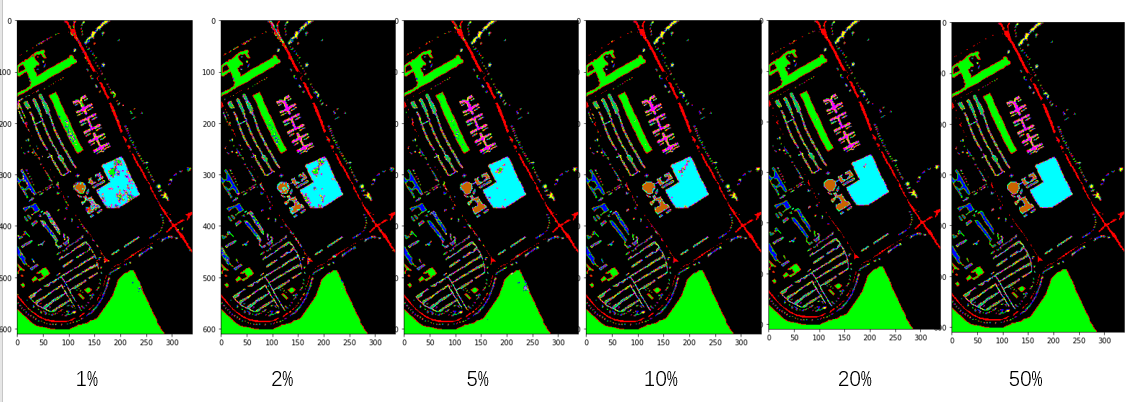
\includegraphics[width = 18cm]{results_multi_feature.png}
\caption{多特征级联高光谱图像分析}
\end{figure}


\section{基于深度学习的高光谱图像分类}
网络的主要架构参考《HybridSN: Exploring 3-D–2-DCNN Feature Hierarchy for Hyperspectral Image Classification》\cite{2020HybridSN},代码复现参考于\cite{Tesera__},其中引入了注意力机制,捕获长序列特征和权重。通过引入3D卷积来捕获深度信息,进而实现同时捕获多个波段的编码的光谱信息和空间信息,来克服二维CNN中无法光谱维度提取特征图中信息,通过将3D-CNN和2D-CNN良好的组合,充分利用光谱信息和空间特征图以达到最好的分类效果。为了进一步提高分类的准确性,同时引入了空间注意力机制和通道注意力机制。
\begin{figure}[htbp]
    \centering
    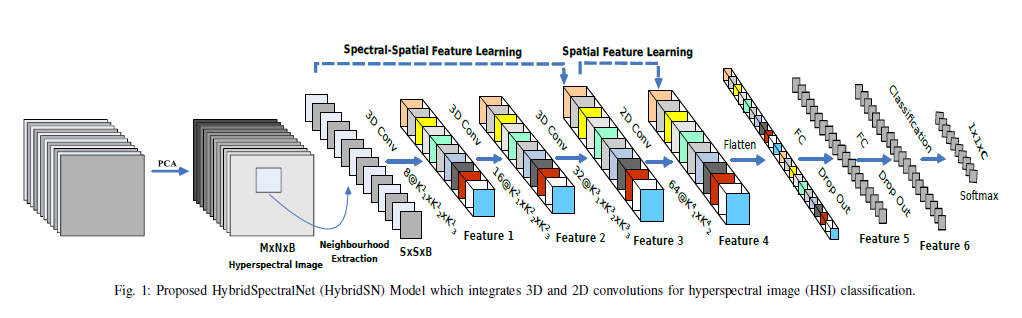
\includegraphics[width=18cm]{20210301104335627.png}
    \caption{网络的主要结构}
    \label{fig:encoder}
\end{figure}

\subsection{光谱维度降维}
由于HybridSN中,输入的channel维度$(B,1,Windows,Window,C)$也就是说在这个基础上,通过不同Patch块的大小以及对应的光谱维度可以获得不同的先验信息,然而上述这两个超参数大小,使得占用的内存成指数倍提升,这里依据笔记本内存的限制,选择光谱维度是20维。
\subsection{Patch图像块的提取}
基于特征工程的高光谱图像分类的处理方法,将原始的图片进行Flatten处理,将生成的光谱维度作为机器学习中传统的特征维度,但是这种处理方法存在的存在的问题是,忽略空域特征中,各个像素之间的联系和结构联系信息,只充分利用了光谱信息等特点。


Patch块的提取方法,利用GT中的标签作为索引,先将图像Pad处理,将整张图四周边缘填充下面对应的行列的像素,随后对于原特征图的每个像素,获取以该像素为中心,Patch块大小的周围像素。为了进一步阐述,我们设定大小为11,张量的维度的变化,见下面的公式2,也就是说送入神经网络,不再是单一二维特征,而是具有空间信息和光谱信息的三维特征。
\begin{equation}
    margin = Round(\frac{Patch Size-1}{2})
\end{equation}
\begin{equation}
    Origin = (42776,103)\qquad
    Transform =(42776,11,11,103)
\end{equation}

\subsection{神经网络的训练}
网络的主体架构同论文中主体一致,为了防止过拟合和加快网络的收敛速度,此次实验中将通道数减少至适中的水平,介绍下几个重要的超参数,训练集和测试集的划分比例是1:9,损失函数的选择为交叉熵损失函数,优化器选择算法是Adam,训练的Epoch为100,batch size 为 128,损失函数的收敛曲线如图所示。

\begin{figure}[t]
\centering  %图片全局居中
\subfigure[卷积神经网络的混淆矩阵图]{
\label{Fig.sub.1}
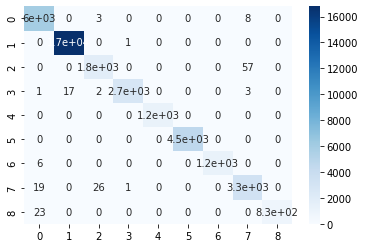
\includegraphics[width=8cm]{model_confusio.png}}\subfigure[HybridSN 网络训练的情况]{
\label{Fig.sub.2}
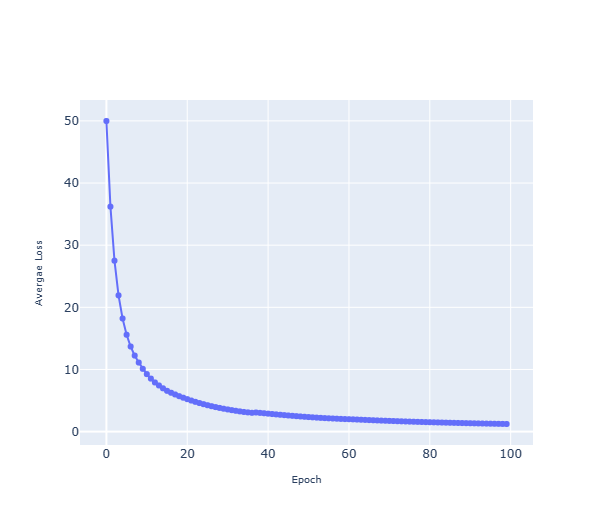
\includegraphics[width=8cm]{newplot (2).png}}
\caption{HybridSN结果图}
\label{1}
\end{figure}

\subsection{模型评估}
通过上面的混淆矩阵表明,网络的训练效果较好,同时在各个指标上超过了基于特征工程的高光谱图像的分类。下面是一些具体的指标,分别是各类评估的准确度,OA,AA,以及Kappa。

% ---- Bibliography ----
%
% BibTeX users should specify bibliography style 'splncs04'.
% References will then be sorted and formatted in the correct style.
%
\begin{table}[]
\caption{基于深度学习高光谱分类的结果}
\label{tab:my-table}
\centering
\setlength\tabcolsep{25pt}
\begin{tabular}{lllll}
\toprule
  & oa       & aa       & kappa    & Tr   \\
  \midrule
0 & 93.86054 & 92.03445 & 91.86144 & 0.99 \\
1 & 96.30018 & 94.44532 & 95.09087 & 0.98 \\
2 & 96.7395  & 96.49564 & 95.71298 & 0.95 \\
3 & 99.40778 & 99.15463 & 99.215   & 0.9  \\
4 & 99.87727 & 99.85729 & 99.83737 & 0.8  \\
5 & 98.75164 & 98.32241 & 98.34355 & 0.5  \\
\bottomrule
\end{tabular}
\end{table}
\begin{table}[]
\centering
\setlength\tabcolsep{10pt}
\caption{深度学习高光谱分类结果维(Each Acc)}
\label{tab:my-table}
\begin{tabular}{llllllllll}
\toprule
  & 0        & 1        & 2        & 3        & 4        & 5        & 6        & 7        & 8        \\
  \midrule
0 & 88.66859 & 98.40411 & 87.89561 & 97.81562 & 99.84733 & 92.30477 & 82.31338 & 85.20693 & 95.85366 \\
1 & 97.02381 & 98.58636 & 74.7486  & 98.82067 & 99.39668 & 97.58888 & 88.3345  & 97.34325 & 98.16514 \\
2 & 99.72607 & 99.95872 & 98.20681 & 96.75151 & 99.29522 & 87.05968 & 99.12837 & 88.66957 & 99.6648  \\
3 & 99.59893 & 99.83932 & 97.12737 & 99.34593 & 100.0    & 99.93369 & 99.83137 & 97.06675 & 99.6483  \\
4 & 99.77431 & 99.96648 & 99.82047 & 99.71405 & 100.0    & 99.97515 & 99.90566 & 99.55947 & 100.0    \\
5 & 99.78935 & 99.0545  & 87.07256 & 99.2228  & 100.0    & 100.0    & 100.0    & 99.76247 & 100.0   \\
\bottomrule
\end{tabular}
\end{table}
\begin{figure}[htbp]
    \centering
    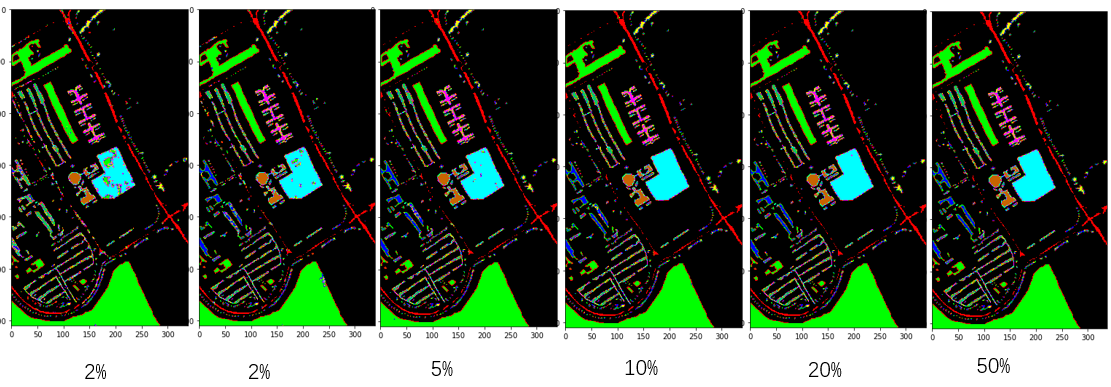
\includegraphics[width=18cm]{Deep_learning_results.png}
    \caption{卷积神经网络输出图像}
    \label{fig:train}
\end{figure}


\section{级联多特征高光谱图像分析与深度学习方法机制的比较}
以机器学习为主要的数据驱动型算法已经自从2012年以后取得巨大的成功,两种力量推动着这种繁荣。硬件方面,定制的GPU集群大大加快算法的运算速度,互联网的快速兴起,基准数据集随着时间推移随着指数化增加。
\subsection{降维的不同的意义}
\\
\subsubsection{卷积神经网络}
卷积神经网络的存在由于较基础的MLP架构,所需要的网络参数大大减小,由于其出色的特征提取能力,在CV领域得到了广泛的应用。回到此次大作业,由于只有单张的图像,但是存在大量的光谱维度。以深度学习传统的机制中,原始的数据不应该被舍弃,反而要应该做数据增强,这步的降维的处理实际上是根据当前的RAM的限制所决定的,由于后续Patch块的提取会挤占大量的内存,以当前PC的16GB为例,当前所选择的参数为该电脑的最大限制。


\subsubsection{多特征级联高光谱图像分类}
在机器学习中,如果存在大量的维度而不进行数据降维的处理,非常容易导致算法的过拟合现象的出现,同时由于大量特征的存在,如果完整的规划、处理、储存特征也是非常的重要的东西。因为没有必要浪费大量的时间和空间去解决大量的垃圾特征。因此,机器学习的特征工程就非常重要,至于后面具体的分类器的模型选择的重要度,则不是那么明显。常见的方法是,将各个特征逐步丢入分类器,如果精度损失不大,则可以停止当前的特征丢弃,来减少维度的数量。多特征级联高光谱降维的算法其实也就是这个,光谱间存在着大量的信息冗余,将其投影到高维度特征后来进一步减少后续特征提取的复杂程度。


\subsection{特征提取方法的优劣}
\subsubsection{特征提取器的问题}
卷积神经的网络可以自动提取便于分类的特征,而传统机器学习方法则更偏向手工提取对应的特征。也就是说前者泛化性好,鲁棒性好。后者主观性大,能动性强。需要调整的超参数太过于多,各个特征提取器之前如果要确定最佳参数,则需要大量的参数,那么如果应用场景发生较大范围改变,之前的一组超参数则没有更多其他维度用处。

\subsubsection{Patch块的问题}
刚才已经提取Patch块的提取过程,Patch块的提取是否针对传统的Tabular的机器学习的过程不公平的问题。因为以当前滑动窗口为例,如果提取单点的像素在区域块的中间,这就会导致一个问题,如果按照正常数据集的分割比例来说,Patch设计虽然提取大量的空间信息,但是多个像素点被得到了复用,也就是说窗口越大拿到的像素数目越多。以1\%分割比例进行计算,深度学习获取的像素实际数量可能小于121倍。这实际上并不符合实际的对比结论。
$$42776\times1\% \times 11\times11$$
\subsubsection{结论分析}
按照实际的对比结果来看,深度学习和级联多特征方法在OA指标上没有明显差异,而在AA中指标中存在大幅度的差异。也就是说,后者在某个单类中的逐像素点分类的效果较高,而存在一个或者多个类赶不上平均指标。一方面是可能是由于特征降维中忽略这个大量的先验信息,另一方面特征提取器并没有获得该类的一些纹理和质地的信息。

\bibliographystyle{splncs04}
\bibliography{biblio}
%
\end{document}
